\documentclass{article}

\newenvironment{proof}{\par \noindent {\bf Proof:}}{\begin{flushright}$\Box$\end{flushright}\par \noindent}
\newtheorem{theorem}{\bf Theorem}
\newtheorem{definition}[theorem]{\bf Definition}
\newtheorem{lemma}{\bf Lemma}
\newtheorem{corollary}[theorem]{\bf Corollary}
\newcommand{\pari}{\hspace{\parindent}}

\usepackage{amsmath}
\usepackage{latexsym}
\usepackage{amssymb}
\usepackage{listings}
\usepackage{tikz}
\usepackage{pdfpages}
%\usepackage{natbib}


\begin{document}

\title{Constrained Optimizaton Modelling on Resource Allocation for Distributed Systems }

\author{Teng Yu}
\date{Fall 2015}

\maketitle
\newpage

\begin{abstract}
{\it The abstract is a very brief summary of the report's contents. It should be about half page long. Somebody unfamiliar with your project should have a good idea of what it is about having read the abstract alone and will know whether it will be of interest to them.}
\\\\
This work intend to improve the performance of resource allocating process on shared hosting cloud platform. We research the relations between different resource allocation requirements and compare with the structure inside the cluster. Then involving order theory and ranking functions to model the allocation and constraints more efficient instead of framing the process as a special Linear Programming formulation\cite{s0}. Finally, we say this approach can be used to extend the work on dynamic workloads.
%Then we propose to consider a constraint-oriented algorithm, named AC3, to reduce the domain of variables before searching
\end{abstract}
$$ $$
\renewcommand{\abstractname}{Acknowledgements}
\begin{abstract}
{\it It is usual to thank those individuals who have provided particularly useful assistance, technical or otherwise, during your project. Your supervisor will obviously be pleased to be acknowledged as they will have invested quite a lot of time overseeing your progress.}
\\\\
Sincere thanks to Dr.Mark Stillwell for his countless helpful comments and advise during this project. Thanks Prof.Alexander Wolf for his supervision. Thanks my personal tutor Dr.Sadri Fariba and my friends in Imperial College for their helps.
\end{abstract}
$$ $$
\newpage
\tableofcontents
$$ $$
{\it This should list the main chapters and (sub) sections of your report. Choose self-explanatory chapter and section titles. If possible you should include page numbers indicating where each chapter/section begins. Try to avoid too many levels of subheading. Try if possible to stick to sections and subsections; subsubsections are usually avoidable.}

\section{Introduction}
{\it This is one of the most important components of the report. It should begin with a clear statement of what the project is about so that the nature and scope of the project can be understood by the reader. It should summarise everything you set out to achieve, provide a clear summary of the project's background and relevance to other work, and give pointers to the remaining sections of the report that contain the bulk of the technical material.}

\section{Background and Related Work}
{\it The background and related work section of the report should set the project into context by relating it to existing published work that you read at the start of the project when your approach and methods were being considered. There are usually many ways of approaching a given problem, and you should not just pick one at random. Describe and evaluate as many alternative approaches as possible. The published work may be in the form of research papers, articles, text books, technical manuals, or even existing software or hardware of which you have had hands-on experience. Do not be afraid to acknowledge the sources of your inspiration; you are expected to have seen and thought about other people's ideas, so your contribution largely will be putting them into practice in some other context.}
$$ $$



\section{Body of report-Original Ideas}
{\it The central part of the report typically consists of three of four chapters detailing the technical work undertaken during the project. The structure of these chapters is highly project dependent. Usually they reflect the chronological development of the project, e.g., design, implementation, experimentation, and optimisation, although this is not always the best approach. However you choose to structure this part of the report, you should make it clear how you arrived at your chosen approach in preference to the other alternatives documented in the background. For implementation projects you should describe and justify the design of your system at some high level, for example by using any of the design methods taught during the first- and second-term courses, and should document any interesting problems with, or features of, your implementation. Integration and testing are also important to describe. Your supervisor will advise you on the most suitable structure for these middle sections.}
$$ $$
\subsection{RArs Relations}
Consider to handle with resource that have difficult-to-represent capacities. User's request may be special on different processing element (heterogeneous)or say the relation between them. Then we find the capacity of a cluster is the set of all allocation request that it can service. Try to give a relation between resource allocation requests(RAr):
\begin{definition}
Given the relation $\preceq$ between RAr:
$$ \forall \alpha \in a\ cluster\ device, \exists A,B \in RAr, such\ that\ A \preceq B\ \Leftrightarrow \alpha{(B)} \mapsto \alpha{(A)}. $$
\end{definition}
We say $\alpha{(B)}$ is true iff $\alpha$ can service B. Then we can define a parallel relation between RArs as follow:
\begin{definition}
$$ \forall A,B \in RAr, A\npreceq B\ \wedge B\npreceq A\ \Leftrightarrow A \parallel B. $$
\end{definition}
Followed by defining relations between user's requests, we can try to build a closed topology involving those requests. It will be more likely a lattice as we can ordered those requests by inclusion through the relation we just defined. As the topology inside a cluster device can be viewed as a littice as well by considering that the intersection of subset servers in cluster, it leads to a possibility to achieve mappings during the allocating process.\\\\ A trivial approach from the order theory is to consider Birkhoff's representation theory, which says modular lattice can be represented by down-sets of its corresponding partial order composed by join-irreducible elements. Then it is easy to view the RArs as downset of the lattice of cluster topology. Then 
it remains to create a metric or say ranking function to compare the performance between different mapping.

\subsection{RArs Model}
Consider there is a common foundation of all RArs which is  a non resource needed request, we represent it as $\bot$. \\\\ 
Say there are some kind of basic RArs which hold only one dimension of resource need. For instance, one RAr, named $A_{1}$, may only need some CPU capacity for computation while another, named $A_{2}$, just need some memory capacity to record information. It is easy to verify that not all cluster devices which can service $A_{1}$ can service $A_{2}$ and vise versa. So in this case, $A_{1}$ and $A_{2}$ are parallel while $\bot$ $\preceq$ $A_{1}$,$A_{2}$. Then it is also easy to extend this instance to the real case that there will be a large number $n$ of different dimensions of RArs, and we have the following two conditions:
$$1)\ \forall i,j \in n, A_{i} \parallel A_{j} $$ 
$$2)\ \forall i \in n, \bot \preceq A_{i}\ \ \ $$
Now we consider the union of those RArs $A_{i}$. Some more complexed RArs may contain multi-dimensional resource allocation requests, which can be viewed as request different one-dimensional RArs simultaneously and this can be achieve by the union of $A_{i}$. In this way, we can define a n-dimensional RAr as follows:
\begin{definition}
Given $A^{n}$ denote a n-dimensional RAr, then:
$$ A^{n} = (\forall A_{i}\ i\in n) \bigwedge A_{i}. $$
\end{definition}
Finally, we say any kind of resource allocation request can be viewed as a n-dimensional RAr and the topology of RArs model can be built up as a partially order set through the relations we just defined. We give an instance of two-dimensional RAr topology in \textbf{Figure \ref{fig:rar}}. We use $A_{1}(1)$ to represent a one-dimensional RAr which only require 1GHz CPU and $A_{2}(1)$ to represent another one-dimensional RAr requiring 1GB memory. Then $A^{2}(1,1)$ is the union of them and represent a two-dimensional RAr. For easy illustration, we suppose 1GHz CPU and 1GB memory are two atom (or say entry) requests in this instance. As there may be 1.5GHz CPU request in a RAr, we use dash line to denote the relation which contains intern nodes and full line to denote the closed relation. It is not a supervise that we find the result topology is actually a modular lattice.\\\\
\begin{figure}
\centering
\begin{tikzpicture}
\node (a0) at (10,2) {$A_{2}(2)$};
\node (a1) at (9,1) {$A_{2}(1)$};
\node (a2) at (8,0) {$\bot$};
\node (a3) at (7,1) {$A_{1}(1)$};
\node (a4) at (6,2) {$A_{1}(2)$};
\node (a5) at (8,2) {$A^{2}(1,1)$};
\node (a6) at (7,3) {$A^{2}(2,1)$};
\node (a7) at (9,3) {$A^{2}(1,2)$};
\node (a8) at (8,4) {$A^{2}(2,2)$};
\node (a10) at (11.5,3.5) {$A_{2}(n)$};
\node (a11) at (10.5,4.5) {$A^{2}(1,n)$};
\node (a20) at (4.5,3.5) {$A_{1}(n)$};
\node (a21) at (5.5,4.5) {$A^{2}(n,1)$};
\node (a100) at (8,7) {$A^{2}(n,n)$};
\draw[dash pattern=on2pt off3pt] (a5) -- (a6);
\draw[dash pattern=on2pt off3pt] (a6) -- (a8);
\draw[dash pattern=on2pt off3pt] (a7) -- (a8);
\draw (a2) -- (a3);
\draw (a2) -- (a1);
\draw[dash pattern=on2pt off3pt] (a4) -- (a3);
\draw[dash pattern=on2pt off3pt] (9,5) -- (a8);
\draw[dash pattern=on2pt off3pt] (7,5) -- (a8);
\draw (a5) -- (a1);
\draw (a5) -- (a3);
\draw (a6) -- (a4);
\draw[dash pattern=on2pt off3pt] (a5) -- (a7);
\draw[dash pattern=on2pt off3pt] (a0) -- (a1);
\draw (a0) -- (a7);
\draw[dash pattern=on2pt off3pt] (a5) -- (a7);
\draw[dash pattern=on2pt off3pt] (a0) -- (a10);
\draw[dash pattern=on2pt off3pt] (a11) -- (a100);
\draw[dash pattern=on2pt off3pt] (a21) -- (a100);
\draw[dash pattern=on2pt off3pt] (a20) -- (a4);
\draw[dash pattern=on2pt off3pt] (a21) -- (a6);
\draw[dash pattern=on2pt off3pt] (a11) -- (a7);
\draw (a10) -- (a11);
\draw (a20) -- (a21);
\end{tikzpicture}
\caption{2-dimensional(CPU, Memory) RAr topology}
\label{fig:rar}
\end{figure}

\noindent{\bf Note:} Instead of the theoretical analysis as above, another way of generating the topology of resource allocation requests, or more generally say {\it informations}, is through real data experiment. One instance of this approach can be refer to [MM00] which tested the web-service requests and also resulted a partially order set. 

\section{Evaluation}
{\it All projects need to contain a serious and careful evaluation of their results. The specifics of the evaluation method (e.g., user study, experiments, formal proof review, etc.) are intrinsic to the nature of the project, so this is something that you must discuss and agree with your supervisor early in the project. Ideally, a presentation of the method and results of your evaluation should be included in its own separate section of the report.}

\section{Conclusions and Future work}
{\it All good projects conclude with an objective evaluation of the project's successes and failures, and suggestions for future work that can take the project further. It is important to understand that there is no such thing as a perfect project. Even the very best pieces of work have their limitations and you are expected to provide a proper critical appraisal of what you have done. Your assessors are bound to spot the limitations of your work and you are expected to be able to do the same.}


\section*{Appendices}
{\it Appendices contain information that is peripheral to the main body of the report. Information typically included are things like program listings, tables, proofs, graphs, or any other material that would break up the theme of the text if it appeared in situ. Large program listings are rarely required, and should be compressed as much as possible, e.g., by printing in multiple columns and by using small font sizes, omitting inessential detail.}
\subsection*{Literature Review}
\subsubsection*{From \cite{s1}:} 
Industrial Background: using virtual machine (VM) technology which can consolidate hardware resources to enable shared hosting platforms. \\\\Main achievement: A formulation of the resource allocation problem in shared hosting platform for static workloads to make decisions when allocating hardware resources to service instances.\\\\
System model:  Show in \textbf{Figure \ref{fig:sit}}
\begin{figure}
\center
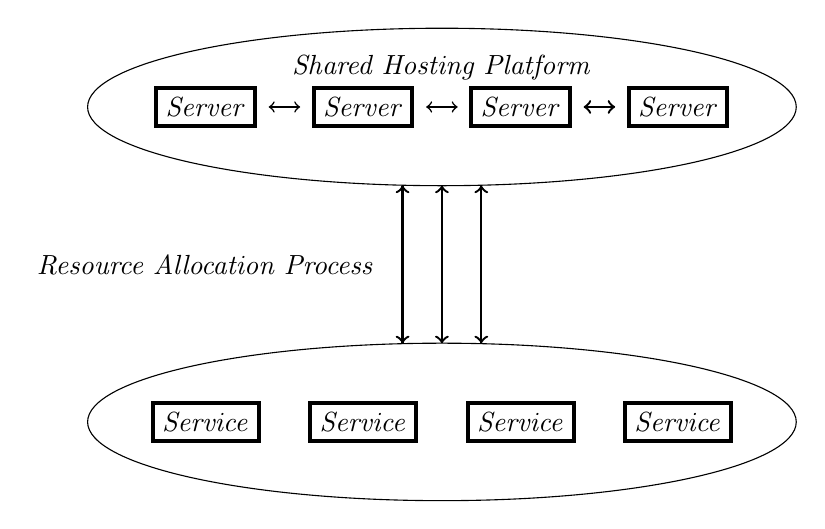
\begin{tikzpicture}
 \node at (3,6.5) {\textit{Shared Hosting Platform}};
\draw (3,2) ellipse (4.5 and 1);
\draw (3,6) ellipse (4.5 and 1);
\node[draw,line width=0.5mm] at (4,6) {\textit{Server}};
\node[draw,line width=0.5mm] at (0,6) {\textit{Server}};
\node[draw,line width=0.5mm] at (2,6) {\textit{Server}};
\node[draw,line width=0.5mm] at (6,6) {\textit{Server}};
\node[draw,line width=0.5mm] at (4,2) {\textit{Service}};
\node[draw,line width=0.5mm] at (0,2) {\textit{Service}};
\node[draw,line width=0.5mm] at (2,2) {\textit{Service}};
\node[draw,line width=0.5mm] at (6,2) {\textit{Service}};
 \draw[<->,line width=0.2mm] (2.8,6) -- (3.2,6);
  \draw[<->,line width=0.2mm] (0.8,6) -- (1.2,6);
   \draw[<->,line width=0.3mm] (4.8,6) -- (5.2,6);
  \draw[->,line width=0.3mm] (3,3) -- (3,5);
  \draw[->,line width=0.3mm] (3,5) -- (3,3);
    \draw[->,line width=0.3mm] (2.5,3) -- (2.5,5);
  \draw[->,line width=0.3mm] (2.5,5) -- (2.5,3);
   \draw[->,line width=0.3mm] (3.5,3) -- (3.5,5);
  \draw[->,line width=0.3mm] (3.5,5) -- (3.5,3);
  \node at (0,4) {\textit{Resource Allocation Process}};
     
\end{tikzpicture}
\caption{System Model} 
\label{fig:sit}
\end{figure}
$$ $$
Resource and Service model: Each server provides several resources (e.g., CPU, RAM space, I/O bandwidth, disk space) and we consider two kinds of resource needs: {\it rigid} and {\it fluid}. A rigid need denotes that a specific fraction of a resource is required.  The service cannot benefit from a larger fraction and cannot operate with a smaller fraction.  A fluid need specifies the maximum fraction of a resource that the service could use if alone on the server. The service cannot benefit from a larger fraction, but can operate with a smaller fraction at the cost of reduced performance. For each fluid resource need we can define the ratio between the resource fraction allocated and the maximum resource fraction potentially used.  We call this ratio the {\it yield} of the fluid resource need. To compare yields across
services with various minimum yield requirements, we define the {\it scaled yield} of a service as follows:
\begin{equation*}
\text{scaled yield} = \frac{\text{yield} - \text{minimum yield}}{1 - \text{minimum yield}}\,.
\end{equation*}

After that, we can specify the assumptions and list them below:\\
1) Each service consists of only a single VM instance.\\
2) Each service has constant resource needs.\\
3) The yields of all fluid resource needs are identical.\\
4) Rigid resource need are independent from fluid resource needs\\
5) User concerns, or say higher level metrics are directly related to resource fractions allocated to services\\\\
Then we specify the aim precisely as {\it Maximize the Minimum Yield} under the two constraints below:\\
1) The resource capacities of the servers not be overcome.\\
2) A service inside a single VM instance should be allocated to a single server.\\\\
%After that, we use the same problem specification and the constraints formulation as a Mixed Integer Linear Program (MILP)\footnote{please refer to page 8 in \cite{s1} for those formulation}.
Finally, we recall the problem formulation as a Mixed Integer Linear Program (MILP). Say we have $N$ services indexed by $i$, $H$ servers indexed by $h$ which each provides $d$ types of resources. Fractions of these resources can be allocated to services. For each service $i$, $r_{ij}$ denotes its resource need for resource type $j$, as a resource fraction between $0$ and $1$. $\delta_{ij}$ is a binary value that is $1$ if $r_{ij}$ is a rigid need, and $0$ if $r_{ij}$ is a fluid need. We use $\hat{y}_{i}$ to denote the minimum yield requirement of service $i$, a value between $0$ and $1$. We define a binary variable $e_{ih}$ that is $1$ if service $i$ runs on server
$h$ and $0$ otherwise. We denote by $y_{ih}$ the unscaled yield of service $i$ on server $h$, which must be equal to $0$ if the service does not run on the server.  With these definitions the constraints of our linear program are as follows, with $Y$ denoting the minimum yield:

\begin{eqnarray}
\forall i,h   & \quad e_{ih} \in \{0, 1\}\;, \quad y_{ih} \in \mathbb{Q} \label{eq.c1}\\
\forall i     & \quad \sum_{h} e_{ih} = 1 \label{eq.c3}\\
\forall i,h   & \quad 0 \leq y_{ih} \leq e_{ih} \label{eq.c4}\\
\forall i     & \quad \sum_{h} y_{ih} \geq \hat{y}_{i} \label{eq.c5}\\
\forall h,j   & \sum_{i} r_{ij} (y_{ih} (1 - \delta_{ij})  + e_{ih} \delta_{ij}) \leq 1 \label{eq.c6}\\
\forall i     & \sum_h y_{ih} \geq \hat{y}_{i} + Y (1 - \hat{y}_i)  \label{eq.c7}
\end{eqnarray}
$$ $$
About Vector Packing Algorithms:
Resource Allocation Problem is related to the multi-dimensional version of bin-packing, or say vector packing: our service may have fluid resource needs. Attempt to place d-dimensional vectors into (at most) H bins.

\subsubsection*{From \cite{r1}:}
A novel approach (Wrasse solver) to resource allocation that permits the problem specification to envelope with ease. The key contribution is defining a specification language for Resource Allocation, which is expressive enough to encode a multitude of allocation problems without using any domain-specific abstractions.\\\\
Face the fact that: there may be conflicting constraints: a strategy that is optimised for performance may not necessarily meet fault-tolerance requirement.

\subsubsection*{From \cite{s0}:}
Focus on the theoretical model: In addition of [Sti10], as heterogeneous cases, we consider each server's each resource (or say node's dimension) has two different capacity: Elementary capacity: a single element in each dimension;  Aggregate capacity: total resource capacity counting all elements.
\\\\
Compared the MILP model with [Sti10]: Using different vector to represent requirement and needs separately instead of invloving a binary indicator. Add one more constraint to represent the aggregate resource capacities achieved by sum the resource used from all services on this node.
\\\\
Still consider the allocation under two constraints: Rigid requirement and fluid need; Both of them become ordered vector pair. Still precisely define the problem as maximize the minimum yield over all services.


\subsubsection*{From \cite{p0} and [Cap01]:}

Notes from Heuristics for Vector Bin Packing [Pan11] 
and Lower bounds and algorithms for the 2-dimensional vector packing problem[Cap01]
--Focus on the new Heuristics and Experiments model, the way to set up the experiment environment.
\\\\
FFD(First Fit Decreasing) Bin-centric view: Open only one bin at any time, place items into this bin from the largest suitable one. Close the bin when no item can be put in. Heuristics: Involve random choosing. Grasp[k]: pick a random one from the best k instead of the bext one. Bubblesearch: the kth best is chosen with a propobability proportional to $(1-p)^k$, for a suitable p.\\\\
Analysis of FFDAvgSum, which is same as VP\_CPSum in\cite{s1}: For the case when some demands in a dimension always dominate the demands in the other dimension, FFDSum is more robust, the dimensions that are not scare can be assigned smaller coefficients and have a smaller impact on the ordering. Analysis \cite{speranza1999oaa}: the demands across the dimensions were simpled i.i.d.
\\\\
Invloving classes of randomly generated instances to model the 2-dimensional case.
Using two variables c,d to represent the bins capacities on different dimensions, respectively.
Using Wj and Vj to represent the weights of item j on different dimensions, respectively.
Using u.d.[a,b] to represent the uniformly distribution of the value for weights of item in the interval [a,b]
\\\\
In [Cap01] and [Pan11], the dimensions in the first six classes are independently sampled.
In classes seven and eight, the dimensions are correlated. They achieve positive correlation by setup the domain
of the Vj to be a monotonic function from Wj while achieve negative correlation by setup it to be a inverse function in domain.
\\\\
In [Pan11]:
Trivial way to extend to multi-dimension is to set dimension (2i-1) and (2i) are correlated as dimension 1 and 2,
while independent of the other dimensions. As for generate negative correlation across all dimensions:
Random variables to denote the random distribution of balls in each dimension, totally 2 times of the dimensions.
Multiply with an random coeffieient from [10,40] and over two (Why?). Further noise by adding a random value from [0,1].
Ignored the overwight item.  

\subsubsection*{From [Van09]:}
This work presents an automatic virtual resource management system for Cloud infrastructures (hosting service platforms). The main advantages include: it can automate the dynamic provisioning and placement of VMs; support for heterogeneous applications and workloads; support for arbitrary application topology.\\\\
Focus on the automatic virtual resource management system:\\\\ 
It contains a more complicate system model, or say architecture, to simulate the resource allocation scenario which is more closed to the really world cloud infrastructures. Instead of using bins and balls to represent, this model composed by Application Environment (AE), Local Decision Module (LDM), Global Decision Module (GDM) and datacenter which contains physical machines and VMs. Briefly, we can say that AE is faced to the application associated with specific performance goals; An application-specific LDM is associated with each AE to evaluate the process baed on the current workload using service-level metric and generate a utility function of the resource allocation; A GDM is used to interact with each LDM and the real-datacenter. It is the core of this system which contains the Constraint solver to determine the management actions based on the input of LDM's utility functions and datacenter's system-level performance metrics. It works like a black box compared with LDM. We prefer to refer to the fig.2 in [Van09] of the system graph.\\\\
Two utility functions in LDM: a fixed service-level function and a dynamic resource-level function which is communicated with GDM and updated for every iteration. VM allocation vectors in LDM are used for build up the upper bound constraints given by each application.\\\\
As for the GDM: It involve two sequential process, one for determine VM allocation vectors for each application (VM Provisioning) and then for placing VMs and PMs and achieving optimisation (VM Packing). Beyond the constraints formulations based on the CPU and Memory, an interesting approach in VM Provisioning is using a coefficient to allow the administrator to trade-off between the fulfilment of the performance goals and the cost of operating the required resources. Another interesting method is illustrated during the optimisation process in VM Packing: To minimise the number of migration required to reach the new VM-to-PM assignment, or say minimise the reconfiguration to provide a strategy with few interim steps and maximum degree of parallelism.  

\section*{User Guide}
{\it For projects that result in a new piece of software, you should provide a proper user guide providing easily understood instructions on how to install and use it. A particularly useful approach is to treat the user guide as a walk through of a typical session, or set of sessions, that collectively display all the features of your software. Technical details of how the software works is rarely required. Keep it concise and simple. The extensive use of diagrams illustrating the software in action prove particularly helpful. The user guide is sometimes included as a chapter in the main body of the report, but is often better as an appendix to the main report.}


%\bibliographystyle{plain}
%\bibliography{biblio}


\begin{thebibliography}{fi99}

\bibitem[Bes06] {b1} C. Bessiere. Constraint Propagation, Chapter 3 of {\it Handbook of Constraint Programming} (eds. Rossi, van Beek and Walsh), Elsevier, 2006.

\bibitem[Bra13] {b2} F. Brandao, J. P. Pedroso. Bin Packing and Related Problems: General Arc-flow Formulation with Graph Compression. {\it Technical Report DCC-2013-08}, Faculdade de Ci�ncias da Universidade do Porto, Portugal. 2013.

\bibitem[Dav02] {d1} B. A. Davey and H. A. Priestley. {\it Introduction to Lattices and Order} Cambridge
University Press, Cambridge, 2002.

\bibitem[Mac85] {mf} A. K. Mackworth and E. C. Freuder. The complexity of some polynomial network consistency
algorithms for constraint satisfaction problems. {\it Artificial Intelligence}, 25:65-74, 1985.

\bibitem[MM00] {bi} Mannila, H; Meek, C. {\it Global Partial Orders from Sequential Data}, Proceedings of sixth ACM SIGKDD international conference on knowledge discovery and data mining, New York, pp161-168, 2000. 

\bibitem[Pan11] {p0} R. Panigrahy, K. Talwar, L. Uyeda, and U. Wieder. Heuristics for Vector Bin Packing {\it Microsoft Research.} 2011

\bibitem[Pro93] {p1} P. Prosser. Hybrid Algorithms for the Constraint Satisfaction Problem, {\it Computational Intelligence}, Volume 9, Issue 3, pp268-299, 1993.

\bibitem[Rai12] {r1} A. Rai, R. Bhagwan, S. Guha. Generalized Resource Allocation for the Cloud {\it Proceedings of the 3rd Symposium on Cloud Computing}. Oct. 2012

\bibitem[Sch04] {semival} M.P. Schellekens, The correspondence between partial metrics and semivaluations, {\it Theoretical Computer Science}, Volume 315, Issue 1, 5 May 2004, 135–149, 2004. 

\bibitem[Sch14] {syrv} M. Schellekens, T. Yu, S. Romaguera, O. Valero, {\it On Semivaluations and Semimodularity} Domains XI International Workshop on domain theory and applications, Paris, France, 2014.

\bibitem[Sti12] {s0} M. Stillwell, F. Vivien, H. Casanova. Virtual Machine Resource Allocation for Service Hosting on Heterogeneous Distributed Platforms {\it IEEE 26th International Parallel and Distributed Processing Symposium}. 2012

\bibitem[Sti10] {s1} M. Stillwell, D. Schanzenbach, F. Vivien, H. Casanova. Resource Allocation Algorithms for Virtualized Service Hosting Platforms. {\it Journal of Parallel and Distributed Computing}. 2010

\bibitem[Sti08] {s2} M. Stillwell, D. Schanzenbach, F. Vivien, H. Casanova. Resource Allocation using Virtual Clusters. Technical Report ICS2008-09-01, Information and Computer Sciences Dept., University of Hawai'i at Manoa, Sept. 2008

\end{thebibliography}


\end{document}



$$ $$
$$ $$
%{\it Keywords: Resource Allocation, Constraint Optimization, Lattices Theory} \\

%\newpage

%\tableofcontents

\section{Problem Statement}
This work intend to extend the results on resource allocation algorithm in \cite{s1}. We try to involve lattices theory to model the constraints more efficient when framing the resource allocation problem for shared hosting platform. %Then we propose to consider a constraint-oriented algorithm, named AC3, to reduce the domain of variables before searching. Finally, we say this approach can be used to extend the work on dynamic workloads.

\subsection{Problem Specification and Formulation}
We recall the problem specification concisely as mentioned in \cite{s1} in this section. We leave the novel-approach description in the next section. The aim of this work is to design an efficient resource allocation system to control how services share the platform. We first provide the background definitions to describe the problem:\\\\
Each server provides several resources (e.g., CPU, RAM space, I/O bandwidth, disk space) and we consider two kinds of resource needs: {\it rigid} and {\it fluid}. A rigid need denotes that a specific fraction of a resource is required.  The service cannot benefit from a larger fraction and cannot operate with a smaller fraction.  A fluid need specifies the maximum fraction of a resource that the service could use if alone on the server. The service cannot benefit from a larger fraction, but can operate with a smaller fraction at the cost of reduced performance. For each fluid resource need we can define the ratio between the resource fraction allocated and the maximum resource fraction potentially used.  We call this ratio the {\it yield} of the fluid resource need. To compare yields across
services with various minimum yield requirements, we define the {\it scaled yield} of a service as follows:
\begin{equation*}
\text{scaled yield} = \frac{\text{yield} - \text{minimum yield}}{1 - \text{minimum yield}}\,.
\end{equation*}
\\\\
After that, we can specify the assumptions and list them below:\\
1) Each service consists of only a single VM instance.\\
2) Each service has constant resource needs.\\
3) The yields of all fluid resource needs are identical.\\
4) Rigid resource need are independent from fluid resource needs\\
5) User concerns, or say higher level metrics are directly related to resource fractions allocated to services\\\\
Then we specify the aim precisely as {\it Maximize the Minimum Yield} under the two constraints below:\\
1) The resource capacities of the servers not be overcome.\\
2) A service inside a single VM instance should be allocated to a single server.\\\\
%After that, we use the same problem specification and the constraints formulation as a Mixed Integer Linear Program (MILP)\footnote{please refer to page 8 in \cite{s1} for those formulation}.
Finally, we recall the problem formulation as a Mixed Integer Linear Program (MILP). Say we have $N$ services indexed by $i$, $H$ servers indexed by $h$ which each provides $d$ types of resources. Fractions of these resources can be allocated to services. For each service $i$, $r_{ij}$ denotes its resource need for resource type $j$, as a resource fraction between $0$ and $1$. $\delta_{ij}$ is a binary value that is $1$ if $r_{ij}$ is a rigid need, and $0$ if $r_{ij}$ is a fluid need. We use $\hat{y}_{i}$ to denote the minimum yield requirement of service $i$, a value between $0$ and $1$. We define a binary variable $e_{ih}$ that is $1$ if service $i$ runs on server
$h$ and $0$ otherwise. We denote by $y_{ih}$ the unscaled yield of service $i$ on server $h$, which must be equal to $0$ if the service does not run on the server.  With these definitions the constraints of our linear program are as follows, with $Y$ denoting the minimum yield:

\begin{eqnarray}
\forall i,h   & \quad e_{ih} \in \{0, 1\}\;, \quad y_{ih} \in \mathbb{Q} \label{eq.c1}\\
\forall i     & \quad \sum_{h} e_{ih} = 1 \label{eq.c3}\\
\forall i,h   & \quad 0 \leq y_{ih} \leq e_{ih} \label{eq.c4}\\
\forall i     & \quad \sum_{h} y_{ih} \geq \hat{y}_{i} \label{eq.c5}\\
\forall h,j   & \sum_{i} r_{ij} (y_{ih} (1 - \delta_{ij})  + e_{ih} \delta_{ij}) \leq 1 \label{eq.c6}\\
\forall i     & \sum_h y_{ih} \geq \hat{y}_{i} + Y (1 - \hat{y}_i)  \label{eq.c7}
\end{eqnarray}


\section{State of the Art}
Resource Allocation Algorithm on shared hosting platforms has been detailed discussed in \cite{s1}. It provided efficient algorithms to handle the resource allocation problem for a static workload of service by modelling as a constraint optimisation problem. A different approach by using arc-flow formulation with graph compression to solve its prototype problem, {\it the bin packing problem}, has been researched and developed recently in \cite{b2}.\\\\
%While, by considering the domain and relation between the constraints, we try to construct lattices to formulate the constraints more efficient (Section 4.1). Then instead of attempting backtracking which had been shown to be unsuccessful in \cite{s2} and having exponential complexity, we propose to involve a polynomial time method, named Arc consistency \cite{b1} to reduce the domains of variables (Section 4.2). We discuss background techniques and provide the knowledge of lattices on Section 2, recall the definitions in \cite{s1} to specify the problem in Section 3, give a general research plan on Section 5 and remark the proposed work on Section 6.  

\subsection{Background Knowledge}
We shortly recall the background knowledge and techniques beyond the resource allocation problem whilst needed for this work. The detail description of the concepts in the section should be refer to \cite{d1,b1,p1}, respectively. 

%\subsection{Set and Lattices Theory}
\begin{definition}
Let $P$ be a set. An partial order on $P$ is a binary relation $\leq$ on $P$ such that, $\forall$ x, y, z $\in$ $P$,\\
(i) x $\leq$ x,
(ii) x $\leq$ y and y $\leq$ x imply x = y,
(iii) x $\leq$ y and y $\leq$ z imply x $\leq$ z.
\end{definition}

\begin{definition}
A set $P$ equipped with an order relation $\leq$ is said to be an partially ordered set. We use the shorthand poset in this paper.
\end{definition}
The cover-relation between elements of a poset  $P$ is defined as follows: $$\forall x,y \in P. \, x \prec y \Leftrightarrow x \leq y \mbox{ and } \not \exists u. \, x \leq u \leq y.$$ We say that ``$y \mbox{ covers }x$'' or ``$x \mbox{ is covered by }y$''. Also, the notation $x \succeq y$ is used to indicate that $x$ covers $y$, or $x$ is equal to $y$. \\

\begin{definition}
Let $X$ be a set. The power-set $\mathcal{Q}$(X), consisting of all subsets of $X$, is ordered by set inclusion: $$ \forall A, B \in \mathcal{Q}(X),\ A\leq B\ if\ and\ only\ if\ A \subseteq B. $$
\end{definition}

\begin{definition}
Let $P$ be a poset and let $S$ $\subseteq$ P. An element x $\in$ $P$ is an upper bound of $S$ if s $\leq$ x for all s $\in$ $S$. A lower bound is defined dually. The least element of the set of all upper bounds of $S$ is called the least upper bound and the greatest lower bound is defined dually as well.
\end{definition}
We use x $\sqcup$ y (read x join y) to represent the least upper bound of \{x,y\}, whilst use x $\sqcap$ y (read x meet y) to represent the greatest lower bound of \{x,y\}. 

\begin{definition}
Let $L$ be a non-empty ordered set. If x  $\sqcup$ y and  x $\sqcap$ y exist for all x, y $\in$ $L$, then $L$ is called a Lattice.\\\\
\end{definition}


%\subsection{Conflict-Directed Backjumping}
%We describe a more efficient "backtrack" technique named Conflict-Directed Backjumping in the subsection. During a searching process through the space, or say move down through a tree, for each variable, we record in a set the variable which caused the conflict for each value we rejected. We pass back the records of all variable conflicts, and add to the conflict set of the variable we are jumping back to. We delete the conflict sets of any variable we are backtracking from or jumping over.
% and Conflict-Directed Backjumping \cite{p1} to reduce the time complexity during the searching process


\section{Key Research Ideas}

%\subsection{Modelling as Lattices}
Instead of defining a 2-D array $e_{ih}$ to indicate the distribution of each service on each server, we only define an array of servers $s_{h}$ and use the values of those variables to indicate the services allocated on it. In another word, the value of the variable for server is a set of numbers. \\\\
The main advantage of this approach is we can represent the original domain of this variable as a lattice [Bottom, Top] composed by inclusion order or more precisely say power-set as mentioned in definition 3. In this case, the Bottom is \{\} means this server not be allocated to any service whilst the Top is \{1,2,...,N\} means this server is allocated to all services. \\\\
Then some constraints can be easily formulated. For instance, we can represent a service only allocated to a single server by: 
$$ \forall h, \sqcap s_{h} = \{ \} $$ Then state the constraint on the yield of service to resource as: $$ \forall i\in s_{h},\ y_{ih}>0 $$ Follow that, we can use the similar formulations as described in MILP in \cite{s1} to achieve the other constraints.

%\subsection{Reducing domain through Arc Consistency}
%We consider the arc consistency through this approach. As mentioned in section 2.2, we can reduce the domain of all variables in the constraint model (using the MILP or the lattice model mentioned above) to optimise the model itself. AC3 algorithm is a typical algorithm which can achieve a polynomial time complexity. We still need a metric, as $dm$ above to implement the algorithm because it will traverse all possible value of the yield one by one to delete the impossible value. This approach is entirely a pre-processing and will not influence the searching algorithm as well. \\\\
It may be not very meaningful(or say useful) under the condition that all the servers are symmetric and can provide all types of resources, but we can still use it to reduce the domains of yields in this case. While on the other hand, it will be very efficient on a special practical scenario which different servers can provide different types and amount of resources. 

%\subsection{For Dynamic Workloads}

\section{Project Work Plan}
We describe the research plan of the above approach in this section.
%\subsection{Modelling as Lattices}
As for modelling the lattices, The first stage is reading the needed materials in detail. There are two parallel work at the next stage. One is to formulate all the constraints needed based on the lattices-model.  We should define a $discrete\ metric$ ($dm$), or say minimum significant bit when formulating the yield as a lattice. For instance,  if we assume $am$ =10\%, the Top in the domain of the yield-lattice will be \{10\%, 20\%,...1\}. Another work in this step may be implementing a prototype programme such as using the lattice-modelling to solve a basic bin packing, or vector packing problem and design a benchmark to compare the performance with a programme implemented by a typical linear-programming model. The results of this testing should be useful to guide the initial modelling process of the real resource allocation problem.\\\\
The next stage will focus on optimize and implement the lattice model. We need to test a suitable $dm$ and implement the constraints by real coding. Many constraint-solver contains a class of set variable, such as the SetVar in Java-Choco. Then, we need another benchmark to compare the performance of this model with the MILP model under the same searching algorithms, say we don't change the searching method in this approach.\\\\
\subsection{Time Schedule}
Oct. - Nov. Reading the needed materials: focus on [Sti10][Sti12], then other references list below.\\
Nov. - Dec. Formulating the new constraint model and first my first report which including the literature review in detail and the description of the new model before the end of this term.\\
Jan. - Feb. Implementing two prototype programme: one to solve basic bin packing by the new model, two to solve the same problem by classical linear model. Compare the performance and analysis the prototype result (technical report).\\
Feb. - Mar. Implementing the programme to solve the vector packing (which is exactly used for resource allocation)by the new model, compare the performance with the programme used in [Sti10], analysis the result (technical report).\\
Mar. - Apr. More test of the programme by large data (on real-distributed platform if possible) and generate the final report.
%\subsection{Reducing domain through Arc Consistency}
%We first need to design a special AC3 algorithm to deal with the resource allocation problem, a more precise pseudo-code based on the algorithm provided in section 2.2. Some possible applications are using it to reduce the domains of the servers/services/yields. As mentioned in above section, we will not apply it to the domain of servers and services if there is a trivial symmetry for the servers.\\\\
%We plan to implement the perudo-code in the next stage and then following the same methods to test and compare the performance as described in the above subsection. 
%\section{Concluding Remarks}
%This proposal contains two novel approaches to extend the work in \cite{s1} on resource allocation problem.\\\\
%If the first approach can work, then we will obtain a total new model to handle the constraint optimisation for resource allocation problem. This modelling method can be extend to solve other problems in distributed system as well in the future. It is easy to say this method will be more efficient for the case when there are a great number of services allocated to only a few but powerful servers or cluster.\\\\
%If the second approach can work,  we can also obtain a more efficient solution even under the same MILP model and the same searching algorithm. This work is suitable for the case when servers provide different type of resource, or say when some resources are useless or limited in some servers. This approach then open a door to extend the work on dynamic workloads, which means instead of re-compute the total resource allocation algorithm each time, we can repeat the AC algorithm to present the changing of resource need. 





%\subsection{Arc Consistency}
%\begin{definition}
%Let $C_{XY}$ be a constraint between two variables X and Y. \\
(i) A pair (v,w) $\in$ $D_{Y}$$\times$$D_{Y}$ is a support for $C_{XY}$, iff (v,w) $\in$ $C_{XY}$\\
(ii) A value v $\in$ $D_{X}$ is arc consistent w.r.t. $C_{XY}$, iff there is a value w $\in$ $D_{Y}$ s.t. (v,w) is a support for $C_{XY}$\\
(iii) $C_{XY}$ is arc consistent iff for every value v $\in$ $D_{X}$, v is arc consistent w.r.t. $C_{XY}$\\
(iv) A Constraint Satisfaction Problem (CSP) = (V,D,C)\footnote{V: the set of variables; D: the domain of each variable; C: the set of constraints} is arc consistent iff for every constraint $C_{ij}$ $\in$ C, $C_{ij}$ and $C_{ji}$ are arc consistent.
\end{definition}
It is easy to say a value which is not arc consistent cannot appear in any solution of a constraint satisfaction problem. Then it is reasonable to consider this consistent before searching and reduce the domains. The trick in this process is when we remove one possible value, other values in other domains may be inconsistent, so we need a efficient method to iterate. \\\\
A common technique for this problem is named $AC3$ and achieved a polynomial-time complexity: $O(ed^{3})$ in which $e$ is the size of the biggest domain and $d$ is the number of constraints \cite{mf}. We provide a pseudo-code for $AC3$ below:\\\\

\begin{lstlisting}[escapechar=@]
@\textbf{AC3}@(V,D,C)
@\textbf{-----------------------------------------------------------------------}@
@\textbf{for}@ each C@$_{XY}$@ in C
    C @$\gets$@ C + {C@$_{XY}$@}  
  Q @$\gets$@ C
@\textbf{while}@ Q @\textbf{$\neq$}@ {}
    C @$\gets$@ dequeue (Q)
    @\textbf{if}@ revise(C@$_{XY}$@) = true
      @\textbf{if}@ D@$_{X}$@ = {}
          @\textbf{return}@ false
       @\textbf{for}@ each C@$_{ZX}$@ in C, Z@\textbf{$\neq$}@Y
          Q @$\gets$@  Q + {C@$_{ZX}$@} 
@\textbf{return}@ true
@\textbf{-----------------------------------------------------------------------}@
\end{lstlisting}
